\chapter{Event reconstruction}\label{chap:reconstruction}

%\chapterquote{}{}

\section{Introduction}

The apparent simplicity --- hits from ionising particles and energy deposits
from particle showers --- and detector granularity of \CMS allows the
reconstruction and identification of muons, electrons and photons, and charged
and neutral hadrons. Instead of simply detecting, reconstructing and
identifying particles with their respective dedicated system an improvement is
made from correlating elements from all detector layers with an attempt to
distinguish all particles by a technique known as particle-flow (PF).

The initial step in reconstruction, prior to the PF method, consists of
forming charged particle tracks from hits in the silicon tracker, tracks in
the muon chambers and calorimeter clusters from energy deposits in the
calorimetry system. The basic building blocks form the input into the PF
algorithm which attempts to link the various blocks into a coherent picture of
a particle candidate. For example, tracks are linked to an \ECAL deposit to
form an electron candidate with further linking to \ECAL deposits consistent
with Bremsstrahlung photons from the electron, which may undergo conversion
resulting in displaced electrons tracks also linked to the primary electron.
Furthermore, the reconstruction of all particles results in a simple \ptmiss
calculation from the negative vector sum of all particle momenta.

This chapter will describe in detail the process of tracking, clustering and
the PF method in the full reconstruction of a proton-proton interaction.


\section{Tracking}

Charged particles originating from the interaction point travel outward
through the magnetic field in helical trajectories. The hits in the silicon
tracker are reconstructed into the track by a fitting procedure known as the
combinatorial track finder.

Hits are formed within the pixel tracker by clustering deposits, above a
certain threshold, in adjacent pixels. The position of the hit for single
pixel clusters is taken at the centre of the pixel while multi-pixel clusters
have a charge-weighted position, correcting for the drift of electrons in the
magnetic field. A more sophisticated, albeit, computationally demanding method
is used for the final track fit which involves a $\chi^2$-fit of expected
charge deposits from a large number of simulated particles through the pixels,
accounting for pixel deterioration, to the observed charge deposit. Strip
tracker hits are formed from clusters of adjacent strips with charge deposits
exceeding a noise-level. The hit position is determined from a charge-weighted
average of the cluster, correcting for the electron drift in the magnetic
field and known inefficiencies with the charge collection. All hits have an
associated uncertainty propagated to the track fitting
procedure~\cite{Chatrchyan:1704291}.

The combinatorial track finder involves a series of Kalman filters (KF)
\cite{Kalman:1960} --- a recursive parameter estimator. A Kalman filter starts
with an initial state (a seed), typically from a guess or estimation,
and iterates across measurements making a prediction and comparing to the
observation to update the initial state, improving the estimation of the
parameters. For track fitting, the fit is performed to five parameters which
describe points along a helical track:
%
\begin{equation}
    \left( \frac{q}{\pt}, x_t, y_t, \theta_t, \phi_t \right)\ \,
\end{equation}
%
where \pt is the transverse momentum of a particle track with charge $q$. The
parameters $x_t$ and $y_t$ are the distances from the interaction point to a
point along the trajectory in the $\vec{x}_t$ and $\vec{y}_t$ axis, shown in
Fig.~\ref{fig:kf_parameters} along with the definitions of the angles
$\theta_t$ and $\phi_t$.

\begin{figure}
    \centering
    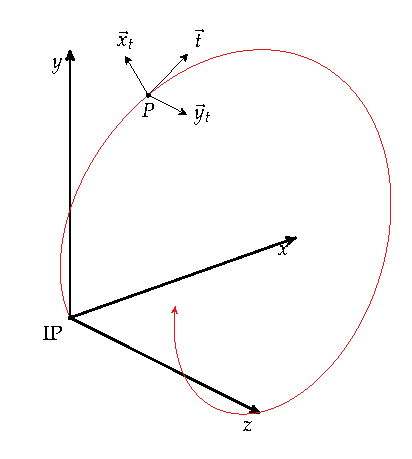
\includegraphics{diagrams/tikz/kf_parameters/kf_parameters.pdf}
    \caption{
        Diagram of a track (shown in red) from the interaction point (IP) with
        the conventional \CMS coordinate system as well as a local coordinate
        system along the trajectory, an example of which is shown at point $P$
        where $\vec{t}$ is the tangential vector, $\vec{x}_{t}$ is
        perpendicular to both the z-axis and $\vec{t}$ and $\vec{y}_{t}$ is
        the remaining vector to create a right-handed coordinate system. The
        angle between the $x$-axis and the projection of ${\vec{t}}$ onto the
        $x$-$y$ plane is $\phi_t$. Similarly, the angle between the $y$-axis
        and the projection of ${\vec{t}}$ onto the $y$-$z$ plane is $\theta_t$.
    }
    \label{fig:kf_parameters}
\end{figure}

The trajectory building with a Kalman filter starts with the seed generation
stage to form guesses for track parameters from a combination of pixel hits,
where the resolution is the greatest and occupancy the lowest. Each iteration
of the Kalman filter extends to the next tracker layer where each hit
candidate, within a $\chi^2$ window, is kept to form independent track
candidates. Fake tacks will typically have a layer where no hits are within
the window and can be dropped. Further checks are performed on the consistency
of hits with the \pt of the track and from vertex constraints. Finally, a
cleaning process assigns unique tracks to a seed and vice versa. After determining the full set of tracks, the Kalman filter procedure is repeated with the precise hit reconstruction, accounting for inter-layer material and field inhomogeneities, with inflated uncertainties to avoid biasing the initial result. Furthermore, the Kalman filter is repeated, seeded by hits from the outermost layer iterating inwards. The best fit tracks are taken from an average of the Kalman filter starting from the inner layers and the reverse.

The trajectory building is performed ten times with different seeds to target
the various classes of tracks with hits associated with candidate tracks
removed from subsequent iterations:
\begin{itemize}
    \item Prompt and high \pt tracks, and $b$-hadron decays are target by the
    first the iterations, seeded by three hits in the pixel detector with
    constraints on the track \pt and distance of nearest approach to the beam axis.
    \item The fourth and fifth iteration target tracks with one or two missing
    hits in the pixel detector as a result of particle interactions and
    decays, or detector inefficiencies. These are seeded by two pixel hits or
    a combination of three pixel and strips hits.
    \item The next two iterations are seeded by strip hits to target displaced tracks.
    \item The eighth iteration targets high \pt jets with merged constituent
    tracks, seeded by pairs of hits in the pixel and strips with the initial
    track compatible with a high energy calorimeter deposit.
    \item The final two iterations are designed to track muons missed by prior
    iterations by using information from the muon chambers to determine the seed.
\end{itemize}
After all iterations are complete a full set of tracks within the tracker
volume are defined, known as inner tracks.


\subsection{Electron tracking}

Electron tracks may be missed by the combinatorial track finder as a result of
significant Bremsstrahlung and high energy photon emission. To recover these
tracks another fitting procedure is performed, based on a gaussian-sum filter
(GSF). The GSF method models hits by a weighted sum of gaussian distributions
for a more accurate representation of hits with sudden and substantial
radiative losses. The results of the expectation fit to the observed hits is
fed into a boosted decision tree\footnote{A boosted decision tree is a form of
supervised learning with an output from a weight linear sum of many decision
trees, optimising a function of the truth and prediction with a regularisation
function to penalise tree complexity.} (BDT) to optimise electron track
reconstruction efficiency while minimising fake tracks. This procedure is also
effective at tracking electron-positron pairs from tracker converted photons.


\subsection{Muon tracking}\label{subsec:muon-tracking}

A track fitting procedure is performed with hits in the muon chambers to form
muon track candidates. Various quality muons are defined based on the inputs
and results of the track fitting:

\begin{itemize}
    \item \textbf{standalone muon:} track fitting seeds are formed of track
    segments from hits within the DT or CSC detectors. The fit itself uses
    hits within all muon chambers.
    \item \textbf{global muon:} a standalone muon track matched to an inner
    track.
    \item \textbf{tracker muon:} one muon segment matched to a unique inner
    track with requirements on the muon's momentum and its compatibility with
    an origin at the beam axis.
\end{itemize}


\section{Calorimeter clustering}

A clustering algorithm groups energy deposits within the calorimeter towers to
encapsulate the whole extend of a particle shower, or multiple overlapping
showers. These clusters are sent to the PF algorithm to link the cluster with
a track, or multiple tracks. The clustering is performed separately in the
ECAL barrel and endcaps, HCAL barrel and endcaps, and the two preshower
layers. No clustering is performed in the HF since forward jets typically have
large momenta and hence collimated showers. Seeds initialise the clustering
and are identified as cells with an energy above a threshold and greater than
the nearest neighbouring cells. Topological clusters are formed by merging
neighbouring cells, with an energy twice the noise level, into the seed cell.
Individual clusters within a topologial cluster are distinguished by a
gaussian-mixture model: a topological cluster in $M$ cells arise from $N$
gaussian energy deposits. The deposits are parameterised by the amplitude of
the {$i$th} gaussian, $A_i$; the position of the gaussian centre in
$\eta$-$\phi$, $\vec{\mu}_i$; and the width $\sigma$ of the gaussian, fixed to
values assigned by each calorimeter system. The initial values are taken from
the cell seeding the topological cluster and an expected energy fraction
measured in cell $j$ is determined from
%
\begin{equation}
    f_{ji} = \frac{A_i\exp\left(-(\vec{c}_i-\vec{\mu}_i)^2/(2\sigma^2)\right)}{\sum_{k=1}^{N}\exp\left(-(\vec{c}_j-\vec{\mu}_k)^2/(2\sigma^2)\right)} ,
\end{equation}
%
where $\vec{c}_i$ is the position of element $i$. The parameters are estimated
from an analytical maximum likelihood fit with
%
\begin{equation}
    A_i & = \sum_{j=1}^{M} f_{ji}E_j
\end{equation}
%
and
%
\begin{equation}
    \vec{\mu}_i & = \sum_{j=1}^{M} f_{ji}E_j\vec{c}_j\ ,
\end{equation}
%
where $E_j$ is the energy deposited in cell $j$. This fit is iterated until
convergence and the position and energy of the gaussian functions are taken as
the cluster parameters.

The energy of the clusters must be calibrated to accurately reflect the true energy deposited. The calibrations are applied independently to electromagnetic and hadronic deposits, reflecting the difference in the corresponding showers. Calibrations are determined from test beam data, radioactive sources, cosmic ray measurements, in situ collision data and simulations.


\section{The particle flow algorithm}

The PF algorithm attempts to resolve all particles from the interaction point
by exploiting the high granularity of the \CMS detector. The algorithm must
deal with particle interactions within the detector leading to crooked tracks
(bent at a `kink') and secondary particles. Furthermore, to avoid a quadratic
computation with the number of particles only the nearest neighbouring PF
blocks in $\eta$-$\phi$ are considered as candidates in the linking algorithm.

The linking of inner tracks to muon tracks has been discussed in
{Sec.~\ref{subsec:muon-tracking}}. Calorimeter clusters are linked to inner
tracks by extrapolating the track to the \ECAL or \HCAL and a linked formed if
these positions lie within a topological cluster's cells, allowing sufficient
margins to account for gaps in calorimeter coverage, shower profile
uncertainties and multiple scattering. A link distance quantifies the distance
between the extrapolated track position and the cluster position in
$\eta$-$\phi$ with the link of minimum distance kept. Bremsstrahlung photons
are linked to electron GSF tracks if tangents, at each tracker layer, to the
track are consistent with \ECAL clusters. A dedicated conversion finder
creates a link between two tracks and a photon if the track are compatible
with the characteristics of a photon conversion. Clusters are linked together
(preshower to \ECAL and \ECAL to \HCAL) if the more granular calorimeter
cluster is within the less granular calorimeter cluster, retaining the link
forming the minimum distance between the two clusters. Finally, tracks are
linked together through a common secondary vertex, attributed to
nuclear-interactions. These tracks must contain at least three tracks: one
incoming from the primary vertex and at least two outgoing, or at least three
outgoing. All links are formed and the subsequent part of the PF algorithm
recovers inefficiencies and removes fake particle candidates by targeting
particular particle classes, as follows.

    
\subsection{Muons}

Global muons are classified as isolated to avoid the misidentification of
charged hadrons, whereby the total energy in a cone of radius ${\Delta
R=\sqrt{\Delta\eta^2+\Delta\phi^2}=0.3}$ around the muon candidate must not
exceed $10\%$ of the muon \pt:
%
\begin{equation}
    I = \frac{1}{\pt}\Biggl(\bigg|\sum_{\substack{i\in \mathrm{tracks}\\\Delta R<0.3}} \vec{p}_{\mathrm{T},i}\bigg| + \sum_{\substack{j\in \mathrm{clusters}\\\Delta R<0.3}}E_{\mathrm{T}}\Biggr) < 0.1\ ,
\end{equation}
%
where $I$ is known as the isolation, $i$ sums the transverse momenta of all
tracks within $\Delta R=0.3$ and $j$ sums the transverse energies of all
clusters within $\Delta R=0.3$. Non-isolated muons are also identified without
the isolation requirement, however, inner tracks must match at least three
track segments in the muon detectors or calorimeter clusters compatible with
the muon hypothesis to avoid high \pt charged hardon misidentification.

The \pt of PF muon candidates is reconstructed from the tracker for
${\pt<\SI{200}{GeV}}$, otherwise the \pt is taken from the track fit resulting
in the lowest $\chi^2$ from the following combinations of information: tracker
only, tracker and the first muon detector plane, global muons and global muons
without high occupancy muon detector planes. After all PF muon candidates are
identified and reconstructed the associated PF blocks are removed from further
candidate identification. Note that under certain conditions charged hadrons
may later be revised as muons.


\subsection{Electrons and isolated photons}

Electron and isolated photon reconstruction must collect and associate
Bremsstrahlung photons and electrons from photon conversions to accurately
measure the true energy of these particles. These secondary particles are
associated to a seed candidate: an \ECAL supercluster above a transverse
energy threshold of ${\SI{10}{GeV}}$ with no GSF track link for photons, or
GSF tracks associated to \ECAL clusters with fewer than three additional
linked tracks. Both classes of candidates must not have \HCAL clusters within
${\Delta R=0.15}$ of the candidate with an energy deposit exceeding $10\%$ of
the supercluster energy. The assigned energy of the candidate is determined
from the sum of all energy deposits linked to the seed, this includes
Bremsstrahlung photons at tangents to GSF tracks at tracker layers and GSF
tracks found by the conversion finder. This energy is calibrated and taken as
the final energy for isolated photon candidates. Electron candidate's energy
is determined from a combination of the calibrated \ECAL energy and GSF track
momentum.

To further reduce misreconstruction the candidates must pass additional
criteria. A BDT is trained separately for the barrel and endcaps, and for
isolated and non-isolated electrons with a requirement placed on the output
determined by the following input features: energy radiated from the GSF
track, distance between the GSF track extrapolation and the \ECAL seeding
cluster, ratio of the \HCAL to \ECAL energy, KF and GSF track $\chi^2$ and the
number of hits in the tracker. Photons, on the other hand, are required to be
isolated from other tracks, calorimeter clusters and have \HCAL to \ECAL
energy ratios consistent with typical photon showers.

Finally, as with muons, the PF blocks associated with the electron and
isolated photon candidates are removed from further processing.


\subsection{Hadrons and non-isolated photons}

The remnants of jet fragmentation and hadronisation with the subsequent decay
of heavy hadrons include: charged hadrons such as $\Ppipm$, $\Pkpm$ and
protons; neutral hadrons such as $\Pklzero$ and neturons; non-isolated photons
typically from $\Ppizero$ decays; and rarely additional muons from early
charged hadron decays. Discrimination of hadrons, other than charged and
neutral, is difficult with high misidentification rates, therefore, the PF
algorithm makes no attempt at this distinction.

From the remaining PF blocks, all \ECAL clusters within the tracker acceptance (${\eta<2.5}$) and no linked tracks are considered as photons. Similarly, \HCAL clusters with the same acceptance and no linked tracks are treated as neutral hadrons.

\begin{itemize}
    \item All ECAL clusters with eta<2.5 with no track link are considered photons and HCAL clusters neutral hadrons. Hadronic jets $25\%$ of energy carried by photons and $3\%$ by neutral hadrons (for taus decays to neutral hadrons are Cabibbo-suppressed lowering this to $1\%$) deposited in ECAL
    \item Beyond 2.5 neutral and charged hadrons cannot be distinguished and leave about $25\%$ of the jet's energy in the ECAL. Precedence to photons is not used here. Therefore, linked ECAL and HCAL clusters are assumed to be from the same charged/neutral hadron shower, while ECAL clusters without links are taken as photons (and calibrated)
    \item Estimated true energy (input into calibrations) taken as:
    \begin{itemize}
        \item ECAL energy for photons
        \item HCAL for hadrons inside the tracker
        \item ECAL+HCAL for hadrons outside
    \end{itemize}
    \item HF EM and HF HAD candidates from depth information and lateral shower profile from comparing 3x3 and 5x5 cluster. These are not calibrated
\end{itemize}

\begin{itemize}
    \item Remaining HCAL clusters are linked to tracks which may also be linked to ECAL clusters
    \begin{itemize}
        \item If calibrated calorimetric energy is in excess of the sum of track momenta significantly larger than the expected calorimetric energy resolution for hadrons -> infers presence of photons and neutral hadrons. If the excess is smaller than the total ECAL energy and largeer than 500 MeV it is identified as a photon with an energy equal to the excess. Otherwise, the recalibrated energy is attributed to a photon and the remaining excess if identified as a neutral hadron (if above 1 GeV)
        \item If calibrated calorimetric energy is compatible with the sum of the track momenta, no neutral particle is identified. Chi2 fit of the tracker and calorimeter measurements redefines charged-hadron pT
        \item Rare cases where calibrated calorimeteric energy is significantly smaller than the sum of track momenta. When larger than three standard deviations - relaxed search for muons (missed previously). If there still exists an excess this is attributed to residual misreconstructed tracks with pT uncertainty in excess of 1 GeV. These are sorted in decreasing pT uncertainty and masked until the momentum excess disappears or no misreconstructed track candidates remain. 
    \end{itemize}
\end{itemize}
    
\begin{itemize}
    \item Nuclear interactions in the tracker material results in secondary charged-particle tracks linked to the secondary vertex. Charged particles are replaced by a single charged hadron with momentum as the vectorial sum of the momenta of secondary charged particles, energy given by sum of energies, and mass set to the charged pion mass. If a well measure momentum of the primary charged particle exists then this is used to estimate energy of undetected secondary particles (not reconstructed as charged or netural particles) to updated the energy of the primary charged hadron
\end{itemize}


\subsection{Event post-processing}

ptmiss
\begin{itemize}
    \item vec(ptmiss,pf(raw)) = -sum particles j(vec(ptj))
    \item Residual small but nonzero probability of particle misidentification and misreconstruction
    \item Rare cases lead to artifically large ptmiss (typically from misidentified or misreconstructed high pt muons)
    \item High pt particles that may lead to a large artrifical ptmiss are selected and the correlation of the particle pt and direction with the ptmiss and direction is determined. Identification and reconstruction of these particles is modified is it can result in a change in ptmiss of at least a half
    \item Muon-related artifical ptmiss:
    \begin{itemize}
        \item Genuine cosmic ray muons in coincidence with an LHC beam crossing. Identified if more than 1cm away from beam axis and removed if ptmiss is reduced. Semileptonic decays of b hadrons rarely reconstructed more than 1 cm away, however, these are protected as the removal would increase the ptmiss instead of decreasing it
        \item Severe muon momentum reconstruction. e.g. Significant difference between available muon momentum estimates. Could be from wrong track association, steel yoke interaction, decay in flight, or synchrotron radiation. PF algo for muons with pT>20 GeV is reviewed. If ptmiss is reduced by half then the momentum estimate that leads to the smallest ptmiss is taken
        \item Particle misidentification. e.g. charged hadron punch-through. This causes energetic neutral hadron deposits in the calorimeters which are wrongly added to the particle list and leads to significant ptmiss (double counting of charged hadron as muon + hadron). If muon momentum and neutral hadron energy are larger than 100 GeV, neutral hadron is removed and muon changed to charged hadron (momentum from inner track), all provided that the ptmiss is reduced by at least one half
        \item Left overs: track/global muon overlaps energetic neutral hadron with similar energy. Then muon candidate is misidentified as charged hadron and neutral hadron disappears leading to ptmiss. Here the test is to turn the charged hadron into a muon and neutral hadron with associated calo energy. Kept if ptmiss reduced by one half
    \end{itemize}
    \item ptmiss is updates as needed
    \item Shown in situ and simulation measurements to not have any considerable effects on real MET events (such at ttbar)
\end{itemize}

%\section{Muon reconstruction}
%
%\section{Electron and photon reconstruction}
%
%\section{Jet reconstruction}
%
%\subsection{$\tau$-tagging}
%
%\subsection{$b$-tagging}
%
%\section{\ptmiss reconstruction}

\section{Summary}

\begin{itemize}
    \item General:
    \begin{itemize}
        \item Particle flow with CMS 2017
        \url{https://arxiv.org/pdf/1706.04965.pdf}
        \item Particle flow and performance of jets, taus, MET 2009
        \url{http://cds.cern.ch/record/1194487}
    \end{itemize}
    \item Lumi:
    \begin{itemize}
        \item Lumi plots in 2016
        \url{https://twiki.cern.ch/twiki/bin/view/CMSPublic/LumiPublicResults#2016_proton_proton_collisions}
    \end{itemize}
    \item Tracking:
    \begin{itemize}
        \item Tracking performance plots in 2016
        \url{https://twiki.cern.ch/twiki/bin/view/CMSPublic/TrackingPOGPlots2016}
    \end{itemize}
    \item EGamma:
    \begin{itemize}
        \item ECAL timing resolution with run 2
        \url{https://cds.cern.ch/record/2682203?ln=en}
        \item Electron and photon performance in 2016
        \url{https://cds.cern.ch/record/2255497/files/DP2017_004.pdf}
    \end{itemize}
    \item Muons:
    \begin{itemize}
        \item Muon HLT performance in 2016
        \url{https://cds.cern.ch/record/2297529/files/DP2017_056.pdf}
        \item Muon reconstruction and performance in 2016
        \url{https://cds.cern.ch/record/2229697?ln=es}
        \item Muon ID and isolation efficiency in 2016
        \url{https://cds.cern.ch/record/2257968?ln=es}
    \end{itemize}
    \item Jets and MET:
    \begin{itemize}
        \item Anti-kt jet clustering 2008
        \url{https://iopscience.iop.org/article/10.1088/1126-6708/2008/04/063}
        \item FASTJET package 2012
        \url{https://link.springer.com/article/10.1140\%2Fepjc\%2Fs10052-012-1896-2}
        \item Jet algorithms performance 2017
        \url{http://cds.cern.ch/record/2622157?ln=en}
        \item Jet energy scale and resolution performance 2018
        \url{http://cds.cern.ch/record/2622157?ln=en}
        \item Performance of MET in 2016
        \url{http://cds.cern.ch/record/2628600?ln=en}
    \end{itemize}
    \item Taus:
    \begin{itemize}
        \item Tau reconstruction and ID in 2016
        \url{http://cms-results.web.cern.ch/cms-results/public-results/publications/TAU-16-003/index.html}
    \end{itemize}
    \item b-tagging:
    \begin{itemize}
        \item Identification in 2016 \url{https://arxiv.org/abs/1712.07158}
        \item Performance in 2016 \url{http://cds.cern.ch/record/2263801?ln=en}
    \end{itemize}
\end{itemize}
